\chapter{Spawning and catching}
\label{chap:spawn}
Pokémon GO is intended to be played on the move.
Trainers primarily interface with the Map screen, onto which is projected
  some approximation of the local geography.
Pokémon spawning on this map will be a Trainer's major source of raw materials.

\textbf{FIXME}

\section{Wild spawns}
\label{sec:spawns}
Decorations around a Pokémon indicate how it spawned (\autoref{table:spawnreasons}).
\begin{table}[ht]
\centering
\begin{tabular}{lll}
  Decoration & Reason for spawn & Visible to\\
\Midrule
  Single white circle & Daily spawn & Trainer\\
  Three white circles & Spawn point & All\\
  Rotating blue spiral & Weather-boosted & All\\
  Pink circles & Incense & Trainer\\
  \textbf{FIXME} & Adventure effect & Trainer\\
  \textbf{FIXME} & Lure & All\\
\end{tabular}
\caption{Spawn decorations}
\label{table:spawnreasons}
\end{table}
Weather-boosted (\autoref{sec:weather}) types enjoy higher spawn rates,
  in addition to higher levels and IVs (\autoref{table:ivfloors}).

\subsection{Lures and incense}
\begin{figure}[h]
\centering
\begin{minipage}[t]{0.3\textwidth}

\includegraphics[width=\textwidth]{images/incense.png}
\caption*{Incense}
\label{fig:incense}
\end{minipage}
\begin{minipage}[t]{0.3\textwidth}

\includegraphics[width=\textwidth]{images/adventureincense.png}
\caption*{Adventure incense}
\label{fig:advincense}
\end{minipage}
\begin{minipage}[t]{0.3\textwidth}
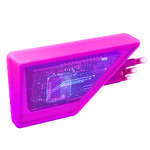
\includegraphics[width=\textwidth]{images/lure.png}
\caption*{Lure module}
\label{fig:lure}
\end{minipage}
\end{figure}
Spawn rates can be increased by means of Incense and Lures.
Incense lasts for an hour, affects only the Trainer using it (i.e.\ other Trainers
  will neither see nor be able to interact with resulting spawns),
  and moves with the Trainer.
A Trainer can make use of only one incense at a time\footnote{The
  ``Mystery Box'', Sunsteel Strike Adventure Effect, and
  Moongeist Beam Adventure Effect similarly cannot be used
  alongside incense, or each other.}.
Incense will result in a spawn every five minutes for immobile Trainers.
Otherwise, incense will result in a spawn every 200 meters moved.
Incense is awarded at certain Trainer levels and for some Research,
  and can be bought for 40 Pokécoins (or eight for 250).

Once unlocked, the Trainer can use Adventure incense.
This special incense results in a greater diversity of spawns, including
  a small chance of the ``Legendary Birds''
  (Galarian Articuno, Galarian Zapdos, and Galarian Moltres).
Adventure incense functions only if the Trainer is moving.
So long as it is completely consumed by midnight, it is automatically replenished
  upon the change of day.
Adventure incense lasts fifteen minutes, so it must be applied before 2345h
  to receive the next day's portion.
Application of Adventure incense grants thirty Poké Balls if the Trainer's
  bag holds fewer than thirty total Poké, Great, and Ultra Balls (\autoref{table:balls}),
  and can accommodate the balls.

Six kinds of Lures (\autoref{table:lures}) can be installed into Pokéstops.
A Pokéstop supports only one lure at a time.
Flower petals will swirl around a Pokéstop with an active lure,
  and also any Pokémon spawned as a result of the lure.
Unlike incense, spawns due to lures are available to all Trainers.
A lure is active for thirty minutes, and then consumed.
Once installed into a Pokéstop, a lure cannot be removed nor deactivated.
Some evolutions (\autoref{sec:evolution}) can only take place near an active lure
 (\autoref{table:condevolutions}).
\begin{table}[ht]
\centering
\begin{tabular}{lcp{.75\textwidth}}
  Lure & Image & Effects\\
  \Midrule
  Lure & 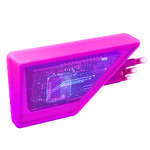
\includegraphics[width=2em]{images/lure.png} & General increase in spawns\\
  Glacial Lure & 
\includegraphics[width=2em]{images/glaciallure.png} & Increased Ice and Water spawns\\
  Magnetic Lure & 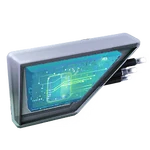
\includegraphics[width=2em]{images/magneticlure.png} & Increased Electric, Rock, and Steel spawns\\
  Mossy Lure & 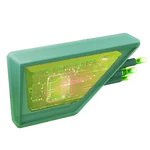
\includegraphics[width=2em]{images/mossylure.png} & Increased Bug, Grass, and Poison spawns\newline Apple drops\\
  Rainy Lure & 
\includegraphics[width=2em]{images/rainylure.png} & Increased Bug, Electric, and Water spawns\\
  Golden Lure & 
\includegraphics[width=2em]{images/goldenlure.png} & Attracts Roaming Form Gimmighoul\newline Gimmighoul Coins from spins \newline Extra items from spins\\
  Mystery Box & 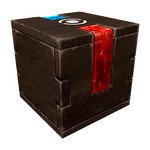
\includegraphics[width=2em]{images/mysterybox.png} & Attracts Meltan\\
\end{tabular}
\caption{Lures and their effects}
\label{table:lures}
\end{table}

\section{Catching}
\label{sec:catch}
Each Pokémon has a catch rate and a flee rate.
\textbf{FIXME}
\subsection{Balls}
\begin{table}[ht]
  \begin{center}
    \begin{tabular}{ll}
      Ball & Effect\\
      \Midrule
      Poké & Standard catch rate\\
      Great & 150\% catch percentage\\
      Ultra & 200\% catch percentage\\
      Master & Guaranteed catch\\
    \end{tabular}
  \end{center}
  \caption{Balls and their properties}
  \label{table:balls}
\end{table}
Raids, Max battles, and Team GO Rocket encounters use special ``Premier Balls''
  rather than the standard options.
Premier Balls cannot be saved after the encounter, and regular balls from
  a Trainer's bag cannot be used in these encounters.
The number of Premier Balls available for an encounter depends on a number of factors \textbf{FIXME}.
Shiny (\autoref{sec:shiny}) raid bosses and Legendary Shadow Pokémon have a 100\% catch rate.

\subsection{Berries}
\label{sec:berries}
\begin{figure}[h!]
  \begin{minipage}[t]{0.3\textwidth}
    \begin{center}
    
\includegraphics[width=\textwidth]{images/razz.png}
    \end{center}
    \caption*{Razz berry}
    \label{fig:razz}
  \end{minipage}
  \begin{minipage}[t]{0.3\textwidth}
    \begin{center}
    
\includegraphics[width=\textwidth]{images/nanab.png}
    \end{center}
    \caption*{Nanab berry}
    \label{fig:nanab}
  \end{minipage}
  \begin{minipage}[t]{0.3\textwidth}
    \begin{center}
    
\includegraphics[width=\textwidth]{images/pinap.png}
    \end{center}
    \caption*{Pinap berry}
    \label{fig:pinap}
  \end{minipage}
\end{figure}
Berries can enhance the catching process (\autoref{table:berries}).
Only one Berry can be applied to a Pokémon at a time.
If a Berry is active, its icon will be shown on the encounter summary.
The Berry is consumed upon use, but persists on the Pokémon across Pokéballs
  and even encounters (i.e., you can leave the encounter, and if you return,
  the Berry will still be applied).
If the Pokémon escapes a Pokéball, however, any applied Berry is gone forever.
A new Berry can be used in this case.
\begin{table}[ht]
\begin{center}
  \begin{tabular}{lp{.75\textwidth}}
Berry & Effect \\
\Midrule
Razz  & 150\% catch percentage\\
Nanab & Immobilizes Pokémon\\
Pinap & Boosts Candy rewards: 3→7, 5→11, 10→23\\
Silver pinap & 180\% catch percentage\newline Boosts Candy rewards: 3→7, 5→11, 10→23\\
Golden razz & 250\% catch percentage\newline Restore full HP to Gym defender\\
\end{tabular}
\end{center}
\caption{Berries and their uses}
\label{table:berries}
\end{table}
\begin{figure}[h!]
  \begin{minipage}[t]{0.5\textwidth}
    \begin{center}
    
\includegraphics[width=\textwidth]{images/silverpinap.png}
    \end{center}
    \caption*{Silver pinap berry}
    \label{fig:silverpinap}
  \end{minipage}
  \begin{minipage}[t]{0.5\textwidth}
    \begin{center}
    
\includegraphics[width=\textwidth]{images/goldenrazz.png}
    \end{center}
    \caption*{Golden razz berry}
    \label{fig:goldenrazz}
  \end{minipage}
\end{figure}

\section{Eggs}
\label{sec:eggs}
\textbf{FIXME}

\section{Shiny Pokémon and other visual forms}
\label{sec:shiny}
Many Pokémon have an alternate presentation known as their ``Shiny'' form.
These forms are collected in their own Pokédex (\autoref{sec:dexen}).
Shadow and Purified Pokémon can be Shiny.
Shininess is preserved across evolution, purification, and trades.
Shininess is not determined at the scope of Pokémon spawns, but for individual
  Trainers' encounters: two Trainers encountering the same spawn might disagree
  on whether or not it is Shiny.
Shiny forms are fairly rare (\autoref{table:shiny}), but various events
  enhance the probability of their generation.
\begin{table}[ht]
\begin{center}
\begin{tabular}{ll}
Context & Probability of shine \\
\Midrule
  Wild spawns & 1/512 (0.195\%) \\
  Team GO Rocket Grunt shadows & 1/256 (0.39\%) \\
  Team GO Rocket Leader shadows & 1/64 (1.56\%) \\
  5🟉 raid & 1/20 (5\%) \\
\end{tabular}
\end{center}
\caption{Likelihood of Shiny Pokémon}
\label{table:shiny}
\end{table}

Despite offering no advantage in battle, and being in no way associated with
  higher levels or IVs, Shiny forms are of great importance to many players.
Personally, unless I expect to trade them, I transfer them to the Professor
  without a second thought.
His usual culinary magic leads to a particularly shiny feast of harvested Pokésoul.
For those determined to collect Shiny forms, the recommended technique
  is to enter as many encounters as possible, check the Pokémon summary
  for the Shiny icon (
\includegraphics[width=1em,keepaspectratio]{images/shiny.png}),
  and exit the encounter immediately if it's absent.

Events sometimes make possible special backgrounds or clothed forms.
Indeed, Froufrou's uselessness in combat is matched only by its
  capacity for wasting Stardust taking on any number of visual forms.

\begin{tcolorbox}[enhanced,title=An aside regarding independent events,halign title=flush center]
\addcontentsline{toc}{section}{An aside regarding independent events}
Let's say a desired result has a 5\% chance of happening, and each event is independent of previous events (like rolls of a fair die, or Shiny status of a 5🟉 raid bonus).\\

\textbf{Q:} How many raids need I do to guarantee at least one Shiny?

\textbf{A:} No finite number of events guarantees the desired result.

\textbf{Q:} OK, but if I do, like, twenty raids, and it's a 5\% chance, it basically has to happen, right?

\textbf{A:} Twenty is sadly finite. 36\% chance of zero gets.

\textbf{Q:} Bullshit, what if I do fifty raids?

\textbf{A:} Fifty is sadly finite. There is about a 7.7\% chance of no love.

\textbf{Q:} My friend got four shiny Pokémon in three raids.

\textbf{A:} That's not a question. It is furthermore untrue.

\textbf{Q:} I'm pretty sure---

\textbf{A:} It's a bullshit patty between two slices of lies is what it is.

\textbf{Q:} Maybe it was four raids.

\textbf{A:} There's a 0.000625\% chance of four wins in four tries. They're independent of your tests,
             so the chance of your friend pulling juice four times in a row while you ate shit given
             the same 5\% chance is 0.000509\%. That's about five times out of a million.
             If you find a lottery offering those odds on the jackpot, well, I'm not saying buy---

\textbf{Q:} Oh shit, does this affect my chance of winning the lottery?\\

Put another way, if you have a 5\% chance of an outcome, and do tests in sets of fourteen,
 over the long term you'll see the outcome in a little over half those sets.
Put yet another way, over the long run, you can expect a little over two Shiny
 Pokémon for every thousand wild spawns.\\

The probability of an outcome with probability $P$ never being seen in $N$ independent
  events is ${(1 - P)}^N$. For a 5\% likelihood, $1 - P = 0.95$. For thirteen events,

  \[ 0.95^{13} ≈ 0.513 \]

There is about a 51.3\% chance that thirteen raids generate no Shiny Pokémon.
\end{tcolorbox}
